%%%%%%%%%%%%%%%%%%%%%%%%%%%%%%%%%%%%%%%%%
% Beamer Presentation
% LaTeX Template
% Version 1.0 (10/11/12)
%
% This template has been downloaded from:
% http://www.LaTeXTemplates.com
%
% License:
% CC BY-NC-SA 3.0 (http://creativecommons.org/licenses/by-nc-sa/3.0/)
%
%%%%%%%%%%%%%%%%%%%%%%%%%%%%%%%%%%%%%%%%%

%----------------------------------------------------------------------------------------
%	PACKAGES AND THEMES
%----------------------------------------------------------------------------------------

\documentclass{beamer}
\usepackage[utf8]{inputenc}
\usepackage{pifont}
\usepackage{svg}
\newcommand{\cmark}{\ding{51}}%
\newcommand{\xmark}{\ding{55}}%
\newcommand{\done}{\rlap{$\square$}{\raisebox{2pt}{\large\hspace{1pt}\cmark}}%
\hspace{-2.5pt}}
\newcommand{\wontfix}{\rlap{$\square$}{\large\hspace{1pt}\xmark}}
\addtobeamertemplate{navigation symbols}{}{%
    \usebeamerfont{footline}%
    \usebeamercolor[fg]{footline}%
    \hspace{1em}%
    \insertframenumber/\inserttotalframenumber
}

\mode<presentation> {

% The Beamer class comes with a number of default slide themes
% which change the colors and layouts of slides. Below this is a list
% of all the themes, uncomment each in turn to see what they look like.

%\usetheme{default}
%\usetheme{AnnArbor}
%\usetheme{Antibes}
%\usetheme{Bergen}
%\usetheme{Berkeley}
%\usetheme{Berlin}
%\usetheme{Boadilla}
%\usetheme{CambridgeUS}
%\usetheme{Copenhagen}
%\usetheme{Darmstadt}
%\usetheme{Dresden}
%\usetheme{Frankfurt}
%\usetheme{Goettingen}
\usetheme{Hannover}
%\usetheme{Ilmenau}
%\usetheme{JuanLesPins}
%\usetheme{Luebeck}
%\usetheme{Madrid}
%\usetheme{Malmoe}
%\usetheme{Marburg}
%\usetheme{Montpellier}%
%\usetheme{PaloAlto}
%\usetheme{Pittsburgh}
%\usetheme{Rochester}
%\usetheme{Singapore}
%\usetheme{Szeged}
%\usetheme{Warsaw}

% As well as themes, the Beamer class has a number of color themes
% for any slide theme. Uncomment each of these in turn to see how it
% changes the colors of your current slide theme.

%\usecolortheme{albatross}
%\usecolortheme{beaver}
%\usecolortheme{beetle}
%\usecolortheme{crane}
\usecolortheme{dolphin}
%\usecolortheme{dove}
%\usecolortheme{fly}
%\usecolortheme{lily}
%\usecolortheme{orchid}
%\usecolortheme{rose}
%\usecolortheme{seagull}
%\usecolortheme{seahorse}
%\usecolortheme{whale}
%\usecolortheme{wolverine}

%\setbeamertemplate{footline} % To remove the footer line in all slides uncomment this line
%\setbeamertemplate{footline}[page number] % To replace the footer line in all slides with a simple slide count uncomment this line

%\setbeamertemplate{navigation symbols}{} % To remove the navigation symbols from the bottom of all slides uncomment this line
}

\usepackage{graphicx} % Allows including images
\usepackage{booktabs} % Allows the use of \toprule, \midrule and \bottomrule in tables
\usepackage{amsmath}
\usepackage{skmath}
\usepackage{csquotes}
\usepackage{datetime}
\usepackage{breakcites}


\ExplSyntaxOn
\RenewDocumentCommand\log{oom}{%
  \IfNoValueTF{#1}
    {\ensuremath{\__skmath_log:\IfNoValueTF{#2}{}{\c_math_superscript_token{#2}}\__skmath_parens:n{#3}}}
    {\ensuremath{\__skmath_log:\c_math_subscript_token{#1}\IfNoValueTF{#2}{}{\c_math_superscript_token{#2}}\__skmath_parens:n{#3}}}%
}
\ExplSyntaxOff

\setbeamertemplate{itemize items}[default]

%----------------------------------------------------------------------------------------
%	TITLE PAGE
%----------------------------------------------------------------------------------------
\title[Text Entailment Seminar] %optional
{An ontology-based approach to model qualitative world knowledge extracted from product reviews for use in QA systems}
\author[]{\Large Thomas Huber\texorpdfstring{\\ \small \vspace{1cm} \color{black}}{ }}
\date[\today] % (optional)
{\today}
\begin{document}
\frame{\titlepage}

\section{Project Description}
\subsection{Project Description}
\begin{frame}{Project Description}
\frametitle{Project Description}
Extend the WordNetGraph \cite{silva2018recognizing} with information about features that certain classes of products have to improve the quality of the graph navigation algorithm and build a basic query system that uses textual entailment to find specific matching products for the query.\\
\\
Which phones take the nicest pictures? $\rightarrow$ Relevant feature is \textit{camera}
\end{frame}

\subsection{Problems}
\begin{frame}{Problems}
    \begin{itemize}
        \item Crawling sufficient amounts of product reviews takes a long time
        \item How to evaluate how / if extending the existing knowledge graph with product features is helpful
        \item Many reviews have spelling errors
        \item How to get from a user query to matching product features
    \end{itemize}
\end{frame}

\subsection{Solutions}
\begin{frame}{Solutions}
    \begin{itemize}
        \item Data: I used an existing dataset of 450212 reviews in the \textit{cellphone} category from Amazon.com \footnote{\url{https://www.kaggle.com/PromptCloudHQ/amazon-reviews-unlocked-mobile-phones/data}, accessed 2018-06-20}
        \item Evaluation: BPI dataset, as used in \cite{silva2018recognizing}, showing new and shorter paths that are created
        \item Spelling errors: Keep only words that appear in the frequency corpus of English Wikipedia \footnote{\url{http://wortschatz.uni-leipzig.de/de/download}, 1 million sentences}
        \item From query to features: Analyze example queries and reformulate them into a textual entailment problem
    \end{itemize}
\end{frame}

\section{Implementation}
\iffalse
    \subsection{Crawler}
    \begin{frame}{Crawler}
    The crawler exists, works, is usable and has been used to extract products. Due to the relatively low speed I then used the aforemention dataset from Kaggle.
    \begin{table}[H]
    \centering
    \caption{Datasets overview}
    \label{table:datasets}
        \begin{tabular}{l|l|l}
        Dataset & number of reviews & number of products \\ \hline
        Drills, own crawler & 36375 & 109 \\ \hline
        Kaggle phone dataset  & 450212 & 4518 
        \end{tabular}
    \end{table}
    \end{frame}
\fi

\subsection{Feature extraction}
\begin{frame}{Feature extraction}
Based on the work by \cite{scaffidi2007red}. Two major changes:
\begin{itemize}
    \item I keep only nouns that appear in the frequency corpus (making the assumption they are correctly spelled if this is the case)
    \item I added a modified score that lowers the score of a feature \textbf{F} for product \textbf{P} if P has only few reviews
\end{itemize}
%
%    \begin{align}
%        \text{Let } l(p) &= \text{number of reviews of product p}\\
%        m(p) &= 
%        \begin{cases}
%            1, \text{if } l(p) \text{ top 50\% \# reviews}\\
%            0.75, \text{if } l(p) \text{ top 90\% \# reviews}\\
%            0.5, \text{if } l(p) \text{ top 95\% \# reviews}\\
%            0.25, \text{if } l(p) \text{ top 99\% \# reviews}\\
%            0.1, \text{otherwise}
%        \end{cases}\\
%        mod\_s(p, f) &= m(p) * s(p, f)
%    \end{align}
%
\end{frame}

\iffalse
\subsection{Extension of the knowledge graph with product features}
\begin{frame}{Extension of the knowledge graph with product features}
Features extracted from products in a category \textbf{C} (currently only \textit{cellphone}) are added to the corresponding node(s) in the existing knowledge graph.
\begin{table}[H]
    \centering
    \caption{RDF example}
    \label{table:rdf-example}
    \begin{tabular}{l|l|l}
        Subject & Predicate & Object \\ \hline
        wnn:cellular\_telephone... & ns1:has\_feature & camera,\\
        & & battery, \\
        &  & screen...
    \end{tabular}
\end{table}
\end{frame}
\fi

\subsection{Graph navigation}
\begin{frame}{Graph navigation}
Based on the work by \cite{silva2018recognizing}.
\begin{itemize}
    \item Start at node \textbf{S}
    \item Get all connected nodes \textbf{N}
    \item Calculate the semantic relatedness between the target \textbf{T} and \textbf{n} $\in$ N (using Indra \cite{indra2018})
    \item If the semantic relatedness is above a threshold, extract the \textit{head words} from the definition of node \textbf{n} and add it to the path so far and add that new path to a stack
    \item A change I made here: If the relation is \textit{supertype}, instead of getting the head words from the definition I use the node itself as the next node
    \iffalse
    ADD EXAMPLE ABOUT APPLE AND FRUIT WHEN TALKING ABOUT THIS
    \fi
\end{itemize}
\end{frame}

\subsection{Usage of product features in graph navigation}
\begin{frame}
    \begin{figure}[H]
        \centering
        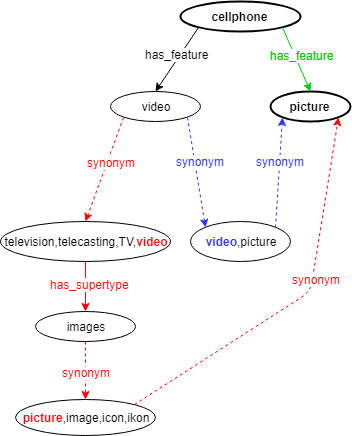
\includegraphics[scale=0.5]{cellphone_navigation.png}
        \caption{Example of three paths found between 'cellphone' and 'picture'}
        \label{fig:cellphone-example}
    \end{figure}
\end{frame}

\subsection{Evaluation}
\begin{frame}{Evaluation}
    \begin{table}[!htb]
    \begin{minipage}{0.7\linewidth}
        \caption{Evaluation on BPI dataset}
        \label{table:bpi-eval}
        \begin{tabular}{llll}
             & Precision & Recall & F1 \\ \hline
            Original & 0.65  & 0.54 & 0.59  \\ \hline
            My system & 0.54 & 0.68 & 0.6 \\
        \end{tabular}
    \end{minipage}%
    \begin{minipage}{0.3\linewidth}
        \centering
        \caption{Confusion matrix for BPI dataset}
        \label{table:bpi-matrix}
        \begin{tabular}{l|llll}
            & Yes &  & No &  \\ \hline
            Yes & 67 &  & 58 &  \\
            No & 31 &  & 93 & 
        \end{tabular}
    \end{minipage}
\end{table}
\begin{table}[!htb]
    \begin{minipage}{.5\linewidth}
        \caption{Evaluation BPI\\ dataset without empty pairs}
        \label{table:bpi-matrix-non-empty}
        \begin{tabular}{llll}
             & Precision & Recall & F1 \\ \hline
             & 0.71 & 0.68 & 0.7 \\
        \end{tabular}
    \end{minipage}%
    \begin{minipage}{.5\linewidth}
        \centering
        \caption{Confusion matrix, BPI\\ dataset without empty pairs}
        \label{table:bpi-eval-non-empty}
        \begin{tabular}{l|llll}
            & Yes &  & No &  \\ \hline
            Yes & 67 &  & \textcolor{red}{27} &  \\
            No & 31 &  & \textcolor{red}{28} & 
        \end{tabular}
    \end{minipage} 
\end{table}
\end{frame}


\subsection{Product recommendation}
\begin{frame}{From query to textual entailment}
    I have formulated a few queries and used dependency parsing to analyze them.
The query and the product features can be transformed into text and hypothesis pairs like so:
\begin{itemize}
    \item Text: A \textit{PRODUCT-CATEGORY} has feature \textit{SOME-FEATURE}.
    \item Hypothesis: A \textit{PRODUCT-CATEGORY} can \textit{TARGET-VERB}.
    \item Hypothesis: A \textit{PRODUCT-CATEGORY} has \textit{TARGET-NOUN}.
\end{itemize}
\end{frame}

\iffalse
    \begin{frame}[plain]{Query dependency parsing example}
     \hspace*{-1.8cm}\parbox[t]{\textwidth}{
        \begin{figure}[H]
            \centering
            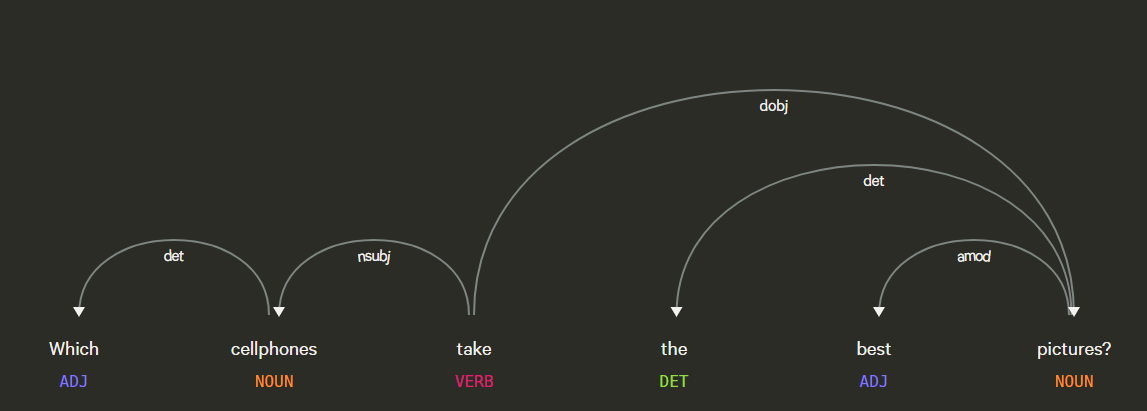
\includegraphics[scale=0.40]{dep-example.PNG}
            \caption{Parse tree example using \url{https://explosion.ai/demos/displacy}}
            \label{fig:dep-example}
        \end{figure}
    }
    \end{frame}
\fi

\begin{frame}{Feature navigation}
    To find matching features, I look for paths between \textit{PRODUCT-CATEGORY} and the target, which is either a verb or a noun as seen on the previous slide.\\
    I then keep all paths that have \textit{has feature} in them and show all products that have the feature and the scores the products have for those features.
\end{frame}

\begin{frame}[plain]{Product recommendation example}
 \hspace*{-1.8cm}\parbox[t]{\textwidth}{
    \begin{figure}[H]
        \centering
        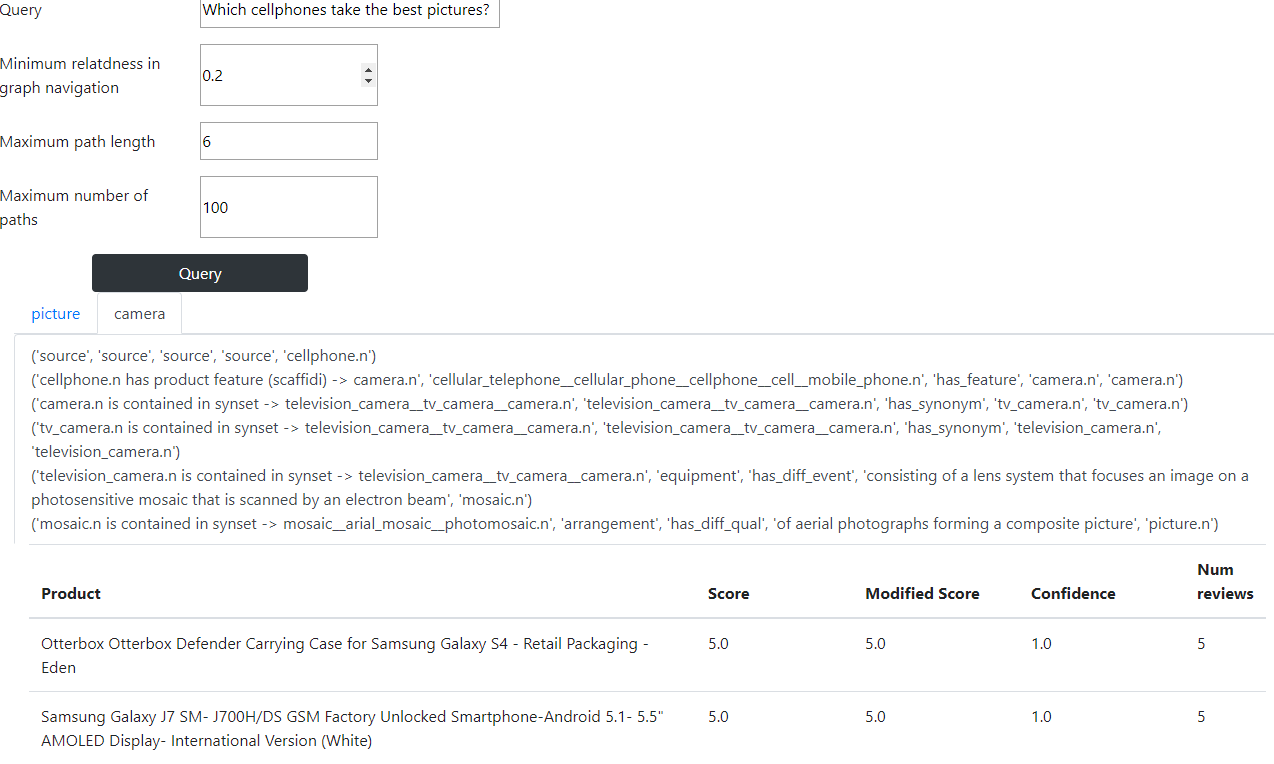
\includegraphics[scale=0.4]{query-example.PNG}
        \caption{Example query and result}
        \label{fig:query-example}
    \end{figure}
}
\end{frame}

\section{Summary}
\begin{frame}{Summary}
\begin{itemize}
    \item Extended existing WordNet knowledge graph with features extracted from Amazon reviews
    \item This creates new paths for the graph navigation algorithm or shortens existing ones
    \item My system produces good results for entailment pairs it can check (precision of 0.71)
    \item Product recommendation component is very basic and can be extended
    \item One option to extend it is to explicitly create entailment pairs and return a list of features matching for a query
\end{itemize}
\end{frame}

\begin{frame}[allowframebreaks]{Bibliography}
\bibliographystyle{plainnat}
\bibliography{references}
\end{frame}

\end{document}